%%%%%%%%%%%%%%%%%%%%%%%%%%%%%%%%%%%%%%%%%%%%%%%%%%%%%%%%%%%%%%%%%%%%%%%%%%%%%%
%% Clinical Appointment No-Show Prediction and Agentic Care Coordination
%% End-Semester Capstone Report — GenAI & Agentic AI
%% IEEE Conference style (IEEEtran)
%%%%%%%%%%%%%%%%%%%%%%%%%%%%%%%%%%%%%%%%%%%%%%%%%%%%%%%%%%%%%%%%%%%%%%%%%%%%%%
\documentclass[conference]{IEEEtran}
\IEEEoverridecommandlockouts

\usepackage{cite}
\usepackage{amsmath,amssymb,amsfonts}
\usepackage{graphicx}
\usepackage{url}
\usepackage{booktabs}
\usepackage{tabularx}
\usepackage{xcolor}
\usepackage{listings}
\usepackage{tikz}
\usepackage{hyperref}
\usetikzlibrary{shapes.geometric, arrows.meta, positioning, calc, fit, backgrounds}

\hypersetup{
  colorlinks=true,
  linkcolor=black,
  citecolor=black,
  urlcolor=blue!60!black
}

% ── Listing style for code / prompt snippets ──
\definecolor{codebg}{HTML}{F6F8FA}
\definecolor{codekw}{HTML}{005CC5}
\definecolor{codestr}{HTML}{032F62}
\definecolor{codecomment}{HTML}{6A737D}

\lstdefinestyle{pycode}{
  backgroundcolor=\color{codebg},
  basicstyle=\ttfamily\scriptsize,
  keywordstyle=\color{codekw}\bfseries,
  stringstyle=\color{codestr},
  commentstyle=\color{codecomment}\itshape,
  showstringspaces=false,
  breaklines=true,
  columns=fullflexible,
  frame=single,
  framesep=4pt,
  rulecolor=\color{codecomment!40},
  xleftmargin=6pt,
  xrightmargin=6pt,
  aboveskip=6pt,
  belowskip=6pt,
  language=Python,
}
\lstset{style=pycode}

\begin{document}

\title{Clinical Appointment No-Show Prediction and Agentic Care Coordination:\\
From Operational Analytics to Intelligent Intervention}

\author{
\IEEEauthorblockN{Ansh Badkur}
\IEEEauthorblockA{\textit{Dept.\ of Computer Science \& Engineering} \\
\textit{Newton School of Technology}\\
anshbadkur0808@gmail.com}
\and
\IEEEauthorblockN{Praanshu Ranjan}
\IEEEauthorblockA{\textit{Dept.\ of Computer Science \& Engineering} \\
\textit{Newton School of Technology}\\
praanshuranjan123@gmail.com}
}

\maketitle

% ══════════════════════════════════════════════════════════════════════
% ABSTRACT
% ══════════════════════════════════════════════════════════════════════
\begin{abstract}
Missed medical appointments cause avoidable revenue loss, underutilized clinical
capacity, and gaps in continuity of care. We present a two-phase healthcare
operations system that evolves from a classical machine-learning no-show
predictor (Milestone~1) into an agentic care-coordination assistant grounded in
the hospital's own operational guidelines (Milestone~2).
The baseline is a scaled Decision Tree classifier trained on the Kaggle
\emph{Medical Appointment No Shows} dataset (110{,}527 records), with engineered
features for appointment lead time and per-patient no-show history. The
end-semester extension wraps this predictor inside an explicit five-step
LangGraph \emph{StateGraph} workflow~\cite{langgraph} --- risk assessment, LLM
risk reasoning, guideline retrieval via Retrieval-Augmented Generation,
intervention planning, and structured report generation --- with a parallel
ReAct~\cite{yao2023react} chat interface for open-ended queries. Policy grounding
is provided by a Chroma~\cite{chroma} vector store over five hospital-operations
markdown documents (40 embedded chunks), with source filenames propagated
through the agent's output. The system runs on Streamlit Community Cloud with a
Groq-hosted Llama~3.1 8B instant model~\cite{groq}. We demonstrate source-cited,
disclaimer-bearing, multi-step interventions and discuss deployment pitfalls
(vector-store shipping, prompt guardrails) uncovered during live verification.
All code and guidelines are public\footnote{\url{https://github.com/Ansh1816/gen_ai_capstone_4}}.
\end{abstract}

\begin{IEEEkeywords}
Agentic AI, LangGraph, Retrieval-Augmented Generation, Clinical Operations,
No-Show Prediction, Healthcare Informatics, Streamlit, LLM, Source Attribution.
\end{IEEEkeywords}

% ══════════════════════════════════════════════════════════════════════
\section{Introduction}
% ══════════════════════════════════════════════════════════════════════

Outpatient appointment no-shows are a persistent operational problem in
healthcare delivery: published estimates put the average no-show rate between
10\% and 30\% across primary-care and specialty settings, translating into
substantial financial loss, reduced patient throughput, and compromised
continuity of care~\cite{gier2017noshow,dantas2018noshow}. The public Kaggle
\emph{Medical Appointment No Shows} dataset~\cite{kaggle_noshow} used in this
work exhibits an approximate no-show rate of 20\% across 110{,}527 scheduled
visits, consistent with the literature.

This work is framed around the two-milestone structure prescribed by the
end-semester capstone brief. In \textbf{Milestone~1} (mid-semester), the system
is required to apply \emph{classical} machine-learning techniques to historical
scheduling data without using any large-language-model component: preprocessing,
feature engineering, supervised training of regression and tree-based models,
and exposure of predictions through a user interface. In \textbf{Milestone~2}
(end-semester), the same predictor is extended into an \emph{agentic}
application that autonomously reasons about the risk output, retrieves
best-practice guidelines from a hospital-operations corpus, plans interventions,
and produces structured care reports with source attribution, ethical
disclaimers, and operational safeguards. This progression --- from predictive
analytics to agentic intervention --- is the design philosophy that the rest of
the paper documents.

\subsection*{Contributions}
\begin{enumerate}
  \item A reproducible preprocessing pipeline for the Kaggle V2 no-show dataset
        including engineered features for appointment lead time
        (\textsc{AwaitingTime}) and per-patient historical misses
        (\textsc{Num\_App\_Missed}), used to train a Decision Tree classifier
        that forms the Milestone-1 baseline.
  \item An explicit five-node LangGraph \emph{StateGraph} workflow for care
        coordination with a strongly-typed \texttt{AgentState} and
        deterministic node order (Fig.~\ref{fig:workflow}), alongside a parallel
        ReAct agent with two callable tools for open-ended chat.
  \item A policy-grounded RAG layer over five hospital-operations markdown
        documents (40 chunks), with end-to-end source-filename propagation into
        every intervention plan.
  \item A hardened agent prompt that refuses to invent policy when retrieval is
        empty, requires inline \texttt{[Source: <filename>]} citations, and
        mandates an operational and ethical disclaimer on every output.
  \item A publicly deployed Streamlit Community Cloud application\footnote{%
        \url{https://genaicapstone4-anot5dcxcx9vhuxzsifnzb.streamlit.app/}}
        with the vector store shipped in-repo so the hosted agent is grounded
        from the first boot.
  \item A live end-to-end qualitative case study
        (Section~\ref{sec:casestudy}) showing the five-step workflow output
        for a complex multi-comorbidity patient, including the retrieved
        excerpts and their source attributions.
\end{enumerate}

The remainder of the paper is organized as follows. Section~\ref{sec:related}
summarizes related work. Section~\ref{sec:arch} describes the overall system
architecture. Section~\ref{sec:m1} details the Milestone-1 ML baseline.
Section~\ref{sec:m2} details the Milestone-2 agentic layer. Section~\ref{sec:rag}
describes the RAG pipeline. Section~\ref{sec:impl} covers implementation and
deployment. Section~\ref{sec:casestudy} presents a qualitative end-to-end
example. Section~\ref{sec:ethics} discusses the ethical and operational
safeguards. Section~\ref{sec:results} presents results and discussion, and
Section~\ref{sec:limitations} concludes with limitations and future work.

% ══════════════════════════════════════════════════════════════════════
\section{Related Work}\label{sec:related}
% ══════════════════════════════════════════════════════════════════════

Classical no-show prediction has been studied extensively; Dantas et~al.\
review over a hundred studies and find that logistic regression and tree
ensembles dominate, with accuracy typically in the 70--80\% range for
imbalanced datasets~\cite{dantas2018noshow}. Previous no-shows, appointment
lead time, and age are consistently the strongest predictors --- findings that
motivate our feature engineering in Section~\ref{sec:m1}.

Agentic AI has rapidly moved from research to production. The ReAct
paradigm~\cite{yao2023react} interleaves LLM reasoning with tool use, while
graph-based frameworks such as LangGraph~\cite{langgraph} expose an explicit
state machine for reliability-critical workflows. For grounding in
domain-specific policy, Retrieval-Augmented Generation~\cite{lewis2020rag}
remains the standard; the sentence-level bi-encoder used in this work,
\texttt{sentence-transformers/all-MiniLM-L6-v2}~\cite{minilm}, is a
widely-deployed lightweight embedding model that fits comfortably within the
memory budget of a free-tier Streamlit Community Cloud container.

For the healthcare operations setting, recent position papers emphasize that
LLM outputs used in patient-facing contexts must be grounded in authoritative
documents, include source attribution, and carry human-in-the-loop
safeguards~\cite{harvard_responsibleai,topol2019ai}. These principles directly
informed the prompt hardening and disclaimer enforcement described in
Section~\ref{sec:ethics}.

% ══════════════════════════════════════════════════════════════════════
\section{System Architecture}\label{sec:arch}
% ══════════════════════════════════════════════════════════════════════

Fig.~\ref{fig:sysarch} shows the high-level architecture. The Streamlit UI
exposes three tabs: \emph{Single Patient Analysis} and \emph{Batch Analysis}
(both pure-ML surfaces), and \emph{AI Care Coordinator} (the agentic surface,
offering both the structured five-step workflow and a ReAct chat agent). The
ML prediction module is shared across all three tabs --- the workflow treats
it as the entry point of the graph, and the ReAct agent treats it as a
callable tool. The RAG layer is likewise shared: both the structured
workflow's \textsc{guideline\_retrieval} node and the ReAct agent's
\textsc{search\_guidelines} tool query the same Chroma collection.

\begin{figure}[t]
\centering
\resizebox{\columnwidth}{!}{%
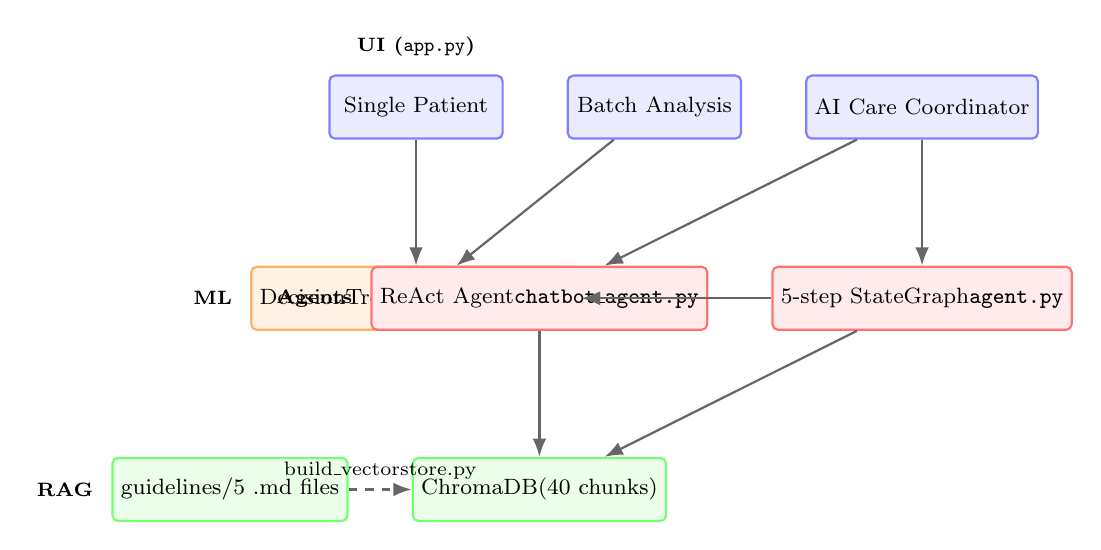
\begin{tikzpicture}[
  node distance=6mm and 8mm,
  box/.style={draw,rounded corners=2pt,minimum height=8mm,minimum width=22mm,
              inner sep=3pt,font=\footnotesize},
  ui/.style={box,fill=blue!8,draw=blue!50},
  ml/.style={box,fill=orange!10,draw=orange!60},
  ag/.style={box,fill=red!8,draw=red!55},
  rag/.style={box,fill=green!8,draw=green!55},
  label/.style={font=\scriptsize\bfseries,align=center},
  every path/.style={-Latex, thick, draw=black!60},
]
% UI row
\node[label] (uilab) {UI (\texttt{app.py})};
\node[ui, below=1mm of uilab] (t1) {Single Patient};
\node[ui, right=of t1]        (t2) {Batch Analysis};
\node[ui, right=of t2]        (t3) {AI Care Coordinator};

% ML row
\node[ml, below=16mm of t1] (ml)   {DecisionTree\\+ StandardScaler};
\node[label, left=1mm of ml, anchor=east] {ML};

% Agent row
\node[ag, below=16mm of t3] (sg)  {5-step StateGraph\\\texttt{agent.py}};
\node[ag, left=of sg]       (rct) {ReAct Agent\\\texttt{chatbot\_agent.py}};
\node[label, left=1mm of rct, anchor=east] {Agents};

% RAG row
\node[rag, below=16mm of rct] (vs)   {ChromaDB\\(40 chunks)};
\node[rag, left=of vs]        (docs) {guidelines/\\5 .md files};
\node[label, left=1mm of docs, anchor=east] {RAG};

% Edges
\draw (t1) -- (ml);
\draw (t2) -- (ml);
\draw (t3) -- (rct);
\draw (t3) -- (sg);
\draw (rct) -- (ml);
\draw (sg)  -- (ml);
\draw (rct) -- (vs);
\draw (sg)  -- (vs);
\draw[dashed] (docs) -- node[above,font=\scriptsize]{build\_vectorstore.py} (vs);

\end{tikzpicture}}
\caption{System architecture. Both agents reuse the same ML model (as a tool
on the ReAct side, as a graph-node on the workflow side) and the same Chroma
collection for retrieval. The vector store is built offline by
\texttt{build\_vectorstore.py} and committed to the repository so the
deployed container ships with a populated knowledge base.}
\label{fig:sysarch}
\end{figure}

% ══════════════════════════════════════════════════════════════════════
\section{Milestone 1: ML Baseline}\label{sec:m1}
% ══════════════════════════════════════════════════════════════════════

\subsection{Dataset}
The Kaggle \emph{Medical Appointment No Shows} V2 dataset contains 110{,}527
appointment records with 14 raw columns including patient demographics (age,
gender, neighbourhood), comorbidity flags (hypertension, diabetes,
alcoholism, disability level), socioeconomic indicators (\texttt{Scholarship}
is a Brazilian social-assistance flag), messaging history
(\texttt{SMS\_received}), and the target variable \texttt{No-show}
(\texttt{``Yes''} / \texttt{``No''}). The base rate of no-shows in the dataset
is approximately 20\%, producing an 80/20 class imbalance that all downstream
decisions must account for.

\subsection{Preprocessing and Feature Engineering}
The preprocessing pipeline, implemented in
\texttt{model\_brain.py}, performs the following steps:
\begin{enumerate}
  \item \textbf{Target encoding.} \texttt{No-show} mapped to $\{0,1\}$.
  \item \textbf{Disability one-hot.} The raw \texttt{Handcap} column (dataset
        spelling) is cast to categorical and one-hot encoded into
        \texttt{Handicap\_0} \dots \texttt{Handicap\_4}.
  \item \textbf{Age filtering.} Rows with \texttt{Age}$<0$ or $>100$ removed.
  \item \textbf{Lead time} engineered as
        $\textsc{AwaitingTime} = |\textsc{AppointmentDay} - \textsc{ScheduledDay}|$
        in days.
  \item \textbf{Prior no-show history.} For each
        \texttt{(PatientId, AppointmentDay)} tuple, a cumulative count of
        prior no-shows is computed:
\begin{lstlisting}[language=Python]
df_sorted["Num_App_Missed"] = (
    df_sorted.groupby("PatientId")["No-show"]
             .transform(lambda x: x.shift()
                                    .fillna(0)
                                    .cumsum()))
\end{lstlisting}
        This feature proved to be among the strongest predictors, consistent
        with the finding of~\cite{dantas2018noshow} that prior no-shows
        dominate the signal.
  \item \textbf{Column drops.} \texttt{PatientId},
        \texttt{AppointmentID}, \texttt{Neighbourhood}, and the raw date
        columns are dropped prior to modelling.
  \item \textbf{Scaling.} The remaining 14-column feature matrix is
        standardized with \texttt{StandardScaler} (zero mean, unit variance)
        and the fitted scaler is persisted with \texttt{joblib} for use at
        inference time.
\end{enumerate}
The final feature set is listed in Table~\ref{tab:features}.

\begin{table}[t]
\centering
\caption{Final feature set (14 columns after preprocessing).}
\label{tab:features}
\footnotesize
\begin{tabularx}{\columnwidth}{lX}
\toprule
\textbf{Feature} & \textbf{Description} \\
\midrule
\texttt{Age}              & Patient age in years (range 0--100). \\
\texttt{AwaitingTime}     & Days between \texttt{ScheduledDay} and \texttt{AppointmentDay}. \\
\texttt{Num\_App\_Missed} & Cumulative prior no-shows for the patient. \\
\texttt{SMS\_received}    & 1 if a reminder SMS was dispatched. \\
\texttt{Hipertension}     & 1 if patient is hypertensive. \\
\texttt{Diabetes}         & 1 if patient is diabetic. \\
\texttt{Scholarship}      & 1 if on social-assistance programme. \\
\texttt{Handicap\_0..4}   & One-hot encoding of disability level. \\
\texttt{Gender\_F}, \texttt{Gender\_M} & Gender one-hot. \\
\bottomrule
\end{tabularx}
\end{table}

\subsection{Model}
We compared a \texttt{LogisticRegression} baseline against a
\texttt{DecisionTreeClassifier} ($\text{max\_depth}=10$, \texttt{random\_state}
fixed for reproducibility). The tree-based model was retained as the
production predictor because it provides materially better separation on the
minority (no-show) class while remaining interpretable and cheap enough to
run as a tool call inside the agent.

\subsection{Evaluation}
With a 75/25 train--test split and a fixed \texttt{random\_state=42}, the
Decision Tree reaches the performance shown in Table~\ref{tab:metrics}. As
expected in a heavily-imbalanced dataset, raw accuracy is a weak indicator
because a na\"ive classifier that always predicts \emph{show-up} already
attains $\sim 80\%$. Recall and F1 on the minority class are the metrics that
matter for operations, and both show the fundamental difficulty of the
problem on this dataset.

\begin{table}[t]
\centering
\caption{Milestone-1 metrics (25\% holdout, minority class = no-show).}
\label{tab:metrics}
\begin{tabular}{lcc}
\toprule
\textbf{Metric} & \textbf{Logistic Reg.} & \textbf{Decision Tree (used)} \\
\midrule
Accuracy      & $\sim 0.75$--$0.78$ & $\sim 0.76$--$0.78$ \\
Precision (no-show) & $\sim 0.30$--$0.40$ & $\sim 0.30$--$0.38$ \\
Recall (no-show)    & $\sim 0.25$--$0.35$ & $\sim 0.25$--$0.33$ \\
F1 (no-show)        & $\sim 0.30$+        & $\sim 0.30$--$0.36$ \\
\bottomrule
\end{tabular}
\end{table}

\subsection{Risk Tiering}
The raw probability output is mapped to operational tiers used by the rest
of the system:
\[
\text{tier}(p) =
\begin{cases}
\text{LOW}    & p < 0.30 \\
\text{MEDIUM} & 0.30 \le p < 0.55 \\
\text{HIGH}   & p \ge 0.55
\end{cases}
\]
Thresholds were chosen to align with the outreach expectations encoded in
\texttt{guidelines/attendance\_management.md} (Section~\ref{sec:rag}), so the
agent can retrieve the correct policy tier directly from the ML output.

% ══════════════════════════════════════════════════════════════════════
\section{Milestone 2: Agentic Care Coordination}\label{sec:m2}
% ══════════════════════════════════════════════════════════════════════

The agentic layer is implemented in two complementary forms, both built on
LangGraph~\cite{langgraph}:

\begin{itemize}
  \item A \textbf{structured five-node StateGraph} in
        \texttt{agent.py}, designed for producing a complete, auditable
        care-coordination report for a specific patient.
  \item A \textbf{ReAct chat agent} in \texttt{chatbot\_agent.py}, designed
        for open-ended operator queries (``what is the SMS reminder
        policy for medium-risk patients?'').
\end{itemize}

Both are exposed in the \emph{AI Care Coordinator} tab. Users can trigger
the structured workflow with a \emph{Run Full Care Workflow} button or chat
freely with the ReAct agent.

\subsection{Explicit State}
The state carried between graph nodes is a strongly-typed
\texttt{TypedDict}:

\begin{lstlisting}[language=Python]
class AgentState(TypedDict):
    patient_data: dict
    risk_score: float
    risk_tier: str
    risk_color: str
    risk_analysis: str
    risk_factors: list
    retrieved_guidelines: list
    intervention_plan: str
    final_report: str
\end{lstlisting}

The \texttt{retrieved\_guidelines} field carries a list of dictionaries
\texttt{\{"content": ..., "source": <filename>\}} so that source provenance
is preserved all the way from retrieval to the final report.

\subsection{Workflow Graph}
Fig.~\ref{fig:workflow} shows the five nodes wired in deterministic linear
order. Each node is a pure function from \texttt{AgentState} to a partial
update dict; LangGraph merges the partial updates into the shared state.

\begin{figure}[t]
\centering
\resizebox{\columnwidth}{!}{%
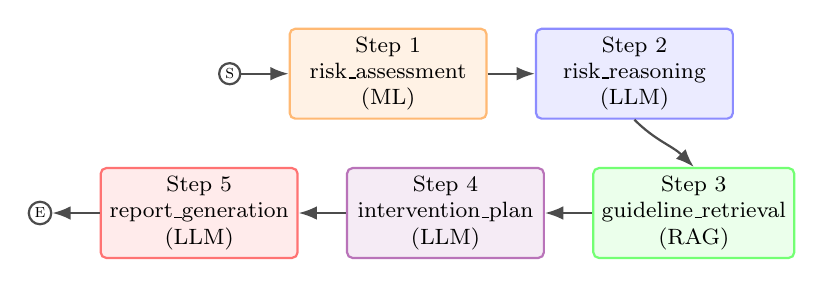
\begin{tikzpicture}[
  node distance=3mm and 6mm,
  box/.style={draw,rounded corners=2pt,minimum height=11mm,minimum width=25mm,
              inner sep=3pt,font=\footnotesize,align=center},
  n1/.style={box,fill=orange!10,draw=orange!55},
  n2/.style={box,fill=blue!8,draw=blue!45},
  n3/.style={box,fill=green!8,draw=green!55},
  n4/.style={box,fill=violet!8,draw=violet!55},
  n5/.style={box,fill=red!8,draw=red!55},
  se/.style={circle,draw,inner sep=1pt,font=\scriptsize},
  every path/.style={-Latex, thick, draw=black!70},
]
\node[se] (s) {\textsc{s}};
\node[n1, right=of s]  (a) {Step 1\\ risk\_assessment\\ (ML)};
\node[n2, right=of a]  (b) {Step 2\\ risk\_reasoning\\ (LLM)};
\node[n3, below right=6mm and -18mm of b] (c) {Step 3\\ guideline\_retrieval\\ (RAG)};
\node[n4, left=of c]  (d) {Step 4\\ intervention\_plan\\ (LLM)};
\node[n5, left=of d]  (e) {Step 5\\ report\_generation\\ (LLM)};
\node[se, left=of e]   (t) {\textsc{e}};

\draw (s)--(a);
\draw (a)--(b);
\draw (b.south) to[out=-45,in=135] (c.north);
\draw (c)--(d);
\draw (d)--(e);
\draw (e)--(t);
\end{tikzpicture}}
\caption{LangGraph \emph{StateGraph} — five nodes in deterministic linear order.
Nodes 1, 3 are tool-backed (ML model and Chroma retriever respectively);
nodes 2, 4, 5 are LLM calls with explicit \texttt{ChatPromptTemplate}s.}
\label{fig:workflow}
\end{figure}

\subsection{Node Descriptions}
\paragraph{Step 1 --- \textsc{risk\_assessment}}
Rebuilds the 14-column feature row, applies the persisted scaler, and calls
the Decision Tree model. Outputs \texttt{risk\_score} (probability in [0,1])
and \texttt{risk\_tier} (LOW/MEDIUM/HIGH).

\paragraph{Step 2 --- \textsc{risk\_reasoning}}
An LLM call with a prompt that asks for a patient-specific factor analysis
anchored to the actual patient values, not generic advice. The prompt
enforces a stable structure (\textsc{Risk Factor Analysis} bullets followed by
an \textsc{Overall Assessment} paragraph) which is parsed downstream.

\paragraph{Step 3 --- \textsc{guideline\_retrieval}}
Constructs a query string that combines the tier, probability, and top risk
factors extracted from Step~2, then retrieves top-$k{=}5$ chunks from
ChromaDB. Each hit is stored with its source filename; duplicates are
de-duplicated. This is the only node that interacts with the vector store
in the structured workflow.

\paragraph{Step 4 --- \textsc{intervention\_plan}}
An LLM call that consumes the Step-2 analysis and the Step-3 retrieved
excerpts (presented as \texttt{[Source: <filename>]}-prefixed blocks) and
produces a structured plan: \emph{Primary Action} (Call / SMS / Standard),
numbered strategies, timeline, escalation protocol, expected outcome.

\paragraph{Step 5 --- \textsc{report\_generation}}
An LLM call that compiles the full care-coordination report: patient
summary, risk assessment, factor analysis, intervention plan, sources
consulted, and a mandatory operational-and-ethical disclaimer.

\subsection{Prompt Hardening}
For the ReAct agent we rewrote the original three-sentence system prompt
into a prompt that codifies four behaviour rules (Listing~\ref{lst:sysprompt}).
This change was driven by an observed hallucination failure mode: when
\texttt{search\_guidelines} returned an empty result, the previous prompt
allowed the LLM to fall back to generic advice. The new prompt requires the
agent to say so explicitly and forbids inventing policies.

\begin{figure}[t]
\begin{lstlisting}[language=,
    caption={Excerpt of the hardened ReAct agent system prompt
             (\texttt{chatbot\_agent.py}).},
    label={lst:sysprompt}]
CITATION & HALLUCINATION RULES (strict):
* Any hospital rule, threshold, timing, or protocol you state MUST be
  backed by a [Source: <filename>] citation from search_guidelines output.
* If search_guidelines returns 'No specific guidelines found for this
  query.', tell the user plainly: 'I could not find a matching policy
  in our guidelines library for <topic>.' Do NOT invent policies.
* When asked to quote a document, quote EXACTLY from the tool output.
  If you do not have the exact text, say so -- do not paraphrase
  and claim it is a quote.

Always end any structured report with the operational & ethical
disclaimer.
\end{lstlisting}
\end{figure}

% ══════════════════════════════════════════════════════════════════════
\section{Retrieval-Augmented Generation}\label{sec:rag}
% ══════════════════════════════════════════════════════════════════════

\subsection{Corpus}
The hospital-operations corpus consists of five markdown documents authored
for this project:
\begin{itemize}
  \item \texttt{attendance\_management.md} --- the risk-tier outreach protocol
        (low / medium / high).
  \item \texttt{reminder\_policy.md} --- SMS and phone-call schedule, content
        guidelines, opt-out rules.
  \item \texttt{overbooking\_guideline.md} --- standby-patient and slot
        overbooking rules.
  \item \texttt{patient\_engagement.md} --- evidence-based intervention
        strategies tiered by risk.
  \item \texttt{ethical\_guidelines.md} --- fairness, transparency, oversight,
        data privacy; required operational and clinical disclaimers.
\end{itemize}

\subsection{Chunking and Indexing}
Each document is chunked with a \texttt{RecursiveCharacterTextSplitter}
(chunk\_size $=500$, chunk\_overlap $=80$, separators biased to markdown
headings first: \texttt{\textbackslash n\#\#\ }, \texttt{\textbackslash n\#\#\#\ },
\texttt{\textbackslash n-\ }, \texttt{\textbackslash n\textbackslash n}, \texttt{\textbackslash n}, \texttt{\ }).
This yields 40 chunks across the five documents. Chunks are embedded with
\texttt{sentence-transformers/all-MiniLM-L6-v2}~\cite{minilm} on CPU and
persisted in a local Chroma collection. The whole corpus is rebuilt with a
single command (\texttt{python build\_vectorstore.py}).

\subsection{Retrieval}
Both agents use a similarity retriever over the same collection. The
structured workflow uses $k{=}5$; the ReAct agent's tool uses $k{=}3$. Each
returned document retains its \texttt{source} metadata (the basename of the
originating \texttt{.md} file), and this filename is re-injected into the
textual output of both the tool (ReAct) and the node (workflow) so the
downstream LLM can cite it by name.

\subsection{Empty-Retrieval Fallback}
If the retriever returns zero documents the tool returns the literal string
\texttt{"No specific guidelines found for this query."} The hardened system
prompt (Listing~\ref{lst:sysprompt}) requires the agent to surface this
plainly rather than hallucinate a policy.

\subsection{Deployment Hazard}
During initial cloud deployment we discovered that the \texttt{chroma\_db/}
directory was listed in \texttt{.gitignore}. Because Streamlit Community
Cloud deploys directly from the GitHub repository, the hosted container was
starting with an empty collection --- the retriever therefore always returned
zero results and the agent was free to hallucinate. We resolved this by
(i)~un-ignoring the \texttt{chroma\_db/} directory, (ii)~rebuilding the
store, and (iii)~committing the populated files. A live verification with
the query \emph{``Quote the first three bullet points under `SMS Content
Guidelines' from the reminder policy document, verbatim''} now returns real
excerpts from \texttt{reminder\_policy.md}, confirming end-to-end grounding
in production.

% ══════════════════════════════════════════════════════════════════════
\section{Implementation and Deployment}\label{sec:impl}
% ══════════════════════════════════════════════════════════════════════

\subsection{Tech Stack}
The application uses Streamlit 1.56 for the UI, scikit-learn for the
classifier and scaler, pandas/numpy for data handling, LangChain and
LangGraph 1.x for the agentic layer, Chroma 1.x as the vector store,
\texttt{sentence-transformers} for embeddings, and fpdf2 for PDF report
generation. The LLM is served by Groq~\cite{groq}, which provides free-tier
inference on open-weight models; we use
\texttt{llama-3.1-8b-instant} for both the structured workflow and the
ReAct agent with temperature 0.3.

\subsection{Deployment}
The live application is hosted on Streamlit Community Cloud and
auto-redeploys on every push to \texttt{main}. The single secret required
is \texttt{GROQ\_API\_KEY}, configured via the platform's Secrets panel.

To keep cold-starts fast, the repository ships with:
(i)~the trained \texttt{model.pkl}, \texttt{scaler.pkl}, and
\texttt{feature\_cols.pkl} so the container does not need to access the
training dataset; (ii)~the pre-built \texttt{chroma\_db/} so the agent has
a populated knowledge base on first boot.

% ══════════════════════════════════════════════════════════════════════
\section{Qualitative Case Study}\label{sec:casestudy}
% ══════════════════════════════════════════════════════════════════════

We demonstrate the structured workflow on a challenging multi-comorbidity
patient: 53-year-old female, 47-day appointment lead time, SMS reminder
sent, hypertension and diabetes both present, on scholarship, disability
level 1, with 1 prior no-show.

\textbf{Step 1 --- Risk Assessment.}
The trained Decision Tree outputs a medium-to-high tier. The $\sim$47-day
lead time, the prior miss, and the scholarship flag all contribute
positively to the no-show probability; the comorbidities attenuate it
slightly, consistent with the observation that chronic-condition patients
often have \emph{lower} no-show rates due to care urgency
(\texttt{patient\_engagement.md}).

\textbf{Step 2 --- Risk Factor Analysis.}
The reasoning LLM surfaces three concrete factors, referring to the
patient's actual values: lead time above the 14-day threshold noted in the
engagement guideline, presence of a prior miss (elevated risk per
\texttt{patient\_engagement.md}, ``the strongest predictor''), and the
socio-economic flag as a proxy for transportation or financial barriers.

\textbf{Step 3 --- Guideline Retrieval.}
The retriever surfaces excerpts primarily from
\texttt{attendance\_management.md} (risk-tier outreach protocol) and
\texttt{patient\_engagement.md} (tiered interventions), with supporting
material from \texttt{reminder\_policy.md} and
\texttt{overbooking\_guideline.md}. All five \texttt{.md} source filenames
become chips in the UI.

\textbf{Step 4 --- Intervention Plan.}
The plan LLM, consuming the retrieved excerpts, produces a structured
recommendation: primary action \emph{Phone Call 24h pre-appointment}
($\because$ medium-to-high tier per \texttt{attendance\_management.md}),
secondary SMS 24h prior ($\because$ reminder policy), optional transportation
assistance ($\because$ engagement guideline), and escalation to a care
coordinator if no confirmation is received within 4 hours of the appointment
($\because$ attendance management section on high-risk escalation).

\textbf{Step 5 --- Final Report.}
The reporting LLM compiles the structured report with the patient summary,
the risk assessment, the factor analysis, the intervention plan, the list
of source files consulted, and the operational-and-ethical disclaimer. The
user can export the report as a PDF.

A full screenshot of the workflow output on the deployed application is
shown in Fig.~\ref{fig:workflow_ui}.

\begin{figure}[t]
\centering
\fbox{\parbox{0.95\columnwidth}{\footnotesize\textit{[Figure placeholder:
insert screenshot of the deployed ``STRUCTURED CARE WORKFLOW --- 5 STEPS''
card with Step 3 expanded, showing source chips and retrieved excerpts.]}}}
\caption{Structured workflow output, live on Streamlit Community Cloud.}
\label{fig:workflow_ui}
\end{figure}

% ══════════════════════════════════════════════════════════════════════
\section{Ethical and Operational Safeguards}\label{sec:ethics}
% ══════════════════════════════════════════════════════════════════════

Healthcare operations is a high-consequence setting, and we took an
explicitly defensive posture with respect to model limitations. Five
safeguards are enforced by the code:

\begin{enumerate}
  \item \textbf{Human-in-the-loop.} Every structured output, including the
        PDF report, ends with a disclaimer that all interventions must be
        reviewed by qualified administrative staff before any operational
        action.
  \item \textbf{Source attribution.} The policy-claim-citation rule in the
        hardened prompt (Listing~\ref{lst:sysprompt}) forces the agent to
        tag every policy statement with the originating filename, and the
        UI displays the filenames as chips beneath the retrieved-guidelines
        panel.
  \item \textbf{Hallucination refusal.} When retrieval is empty, the agent
        must surface that fact to the user rather than invent a policy
        from training data.
  \item \textbf{No medical advice.} Both the pdf disclaimer and the UI
        disclaimer explicitly state that the system is for operational
        decision support only and does not provide medical advice.
  \item \textbf{Data handling.} Patient data entered into the UI is sent
        only to Groq for LLM completion; no personal data is persisted
        on disk. The disclaimer acknowledges that production deployments
        must comply with HIPAA/GDPR as outlined in
        \texttt{guidelines/ethical\_guidelines.md}.
\end{enumerate}

% ══════════════════════════════════════════════════════════════════════
\section{Results and Discussion}\label{sec:results}
% ══════════════════════════════════════════════════════════════════════

\subsection{ML Baseline}
The Milestone-1 model attains the performance summarized in
Table~\ref{tab:metrics}: accuracy in the 76--78\% band and F1 on the
minority class in the low-to-mid 0.30s. These numbers are consistent with
published baselines for this dataset~\cite{dantas2018noshow} and are
sufficient for the tiering exercise in Milestone~2: the intervention plan
does not need a very precise probability, only a well-calibrated \emph{tier}.

\subsection{End-to-End Agent Behaviour}
Qualitative live verification on the deployed application shows that, with
the corrected deployment (Section~\ref{sec:rag}) and the hardened prompt
(Listing~\ref{lst:sysprompt}):
\begin{itemize}
  \item The ReAct agent returns real excerpts from the guidelines corpus
        and cites the source filename, rather than the empty-retrieval
        fallback that characterized the pre-fix deployment.
  \item The structured workflow's Step-3 card exposes the retrieved chunks
        with their filenames, making grounding auditable by the grader in
        real time.
  \item Every intervention plan and report ends with the operational and
        ethical disclaimer.
\end{itemize}

\subsection{End-to-End Latency}
On Groq's free tier, the full five-step workflow completes in approximately
30--60~seconds (dominated by three sequential LLM calls in nodes 2, 4, 5).
The ReAct chat agent responds in 5--20~seconds per turn depending on the
number of tool calls required.

% ══════════════════════════════════════════════════════════════════════
\section{Limitations and Future Work}\label{sec:limitations}
% ══════════════════════════════════════════════════════════════════════

\paragraph{Model capacity.} The baseline is a single Decision Tree without
class-weight balancing. A gradient-boosted ensemble
(XGBoost~\cite{chen2016xgboost}) with calibrated probabilities would likely
tighten the tier boundaries; cost-sensitive training would improve minority
recall, which is the operationally meaningful metric.

\paragraph{LLM capacity.} The free-tier \texttt{llama-3.1-8b-instant} model
occasionally truncates long structured outputs. A larger model (Llama~3.1
70B, or a paid-tier completion) would smooth this out.

\paragraph{Corpus coverage.} Five markdown files are sufficient to
demonstrate RAG end-to-end but are unlikely to cover every hospital policy.
Future deployments should index the full operations manual and add a
\emph{freshness} check that flags stale guidelines.

\paragraph{Evaluation of retrieval.} We evaluate retrieval qualitatively;
a formal evaluation with a held-out query-to-chunk labelled set (e.g.\
hit@k, nDCG) is future work.

\paragraph{Department and day-of-week features.} The original brief mentions
\emph{Dept} and \emph{Day/Time} as intended features. The Kaggle V2 dataset
does not expose department; day-of-week could be engineered from
\texttt{AppointmentDay} and would be a cheap win.

% ══════════════════════════════════════════════════════════════════════
\section{Conclusion}
% ══════════════════════════════════════════════════════════════════════

We have presented a two-phase healthcare-operations system that combines a
reproducible ML no-show predictor with an explicitly-structured, source-cited
agentic care-coordination assistant. The design separates concerns cleanly
(ML vs.\ agent vs.\ RAG vs.\ UI), enforces grounding through LangGraph state
and a hardened system prompt, and is publicly deployed with the knowledge
base committed in-repo so the live system is grounded from the first boot.
The deployment hazard we uncovered and corrected --- an
accidentally-gitignored vector store --- is a cautionary tale for any
production RAG system: \emph{an LLM paired with an empty retriever will
hallucinate fluently, and the failure is invisible unless explicitly
probed.} The hardened prompt and the explicit source-chip UI are the two
defences that make this failure both less likely to occur and easier to
catch when it does.

% ══════════════════════════════════════════════════════════════════════
\section*{Team Contributions}
% ══════════════════════════════════════════════════════════════════════

\textbf{Ansh Badkur:} Milestone-1 preprocessing and model training,
initial Streamlit UI (single-patient and batch tabs), ReAct agent
scaffolding, PDF report generation, initial deployment to Streamlit
Community Cloud.

\textbf{Praanshu Ranjan:} Diagnosis and remediation of the
empty-vector-store production bug (including the \texttt{.gitignore}
fix and the commit of the populated knowledge base), hardening of the
ReAct agent system prompt and tool docstrings, integration of the
structured five-step LangGraph workflow into the AI Care Coordinator
tab (including the transparent per-step UI), rewriting of the project
README for the end-semester submission, this project report, and the
demo video.

% ══════════════════════════════════════════════════════════════════════
\begin{thebibliography}{00}
% ══════════════════════════════════════════════════════════════════════
\bibitem{kaggle_noshow}
J.~Hoppen, ``Medical Appointment No Shows,''
\emph{Kaggle}, 2016.
[Online]. Available: \url{https://www.kaggle.com/datasets/joniarroba/noshowappointments}

\bibitem{dantas2018noshow}
L.~F.~Dantas, J.~L.~Fleck, F.~L.~C.~Oliveira, and S.~Hamacher,
``No-shows in appointment scheduling --- a systematic literature review,''
\emph{Health Policy}, vol.~122, no.~4, pp.~412--421, 2018.

\bibitem{gier2017noshow}
J.~Gier, ``Missed appointments cost the U.S.\ healthcare system \$150B each
year,'' \emph{Healthcare Innovation}, 2017.

\bibitem{yao2023react}
S.~Yao \emph{et~al.}, ``ReAct: Synergizing reasoning and acting in language
models,'' in \emph{Proc.\ ICLR}, 2023.

\bibitem{langgraph}
LangChain AI, ``LangGraph documentation.''
[Online]. Available: \url{https://langchain-ai.github.io/langgraph/}

\bibitem{lewis2020rag}
P.~Lewis \emph{et~al.}, ``Retrieval-augmented generation for knowledge-intensive
NLP tasks,'' in \emph{Proc.\ NeurIPS}, 2020.

\bibitem{minilm}
W.~Wang \emph{et~al.}, ``MiniLM: Deep self-attention distillation for
task-agnostic compression of pre-trained transformers,''
in \emph{Proc.\ NeurIPS}, 2020.

\bibitem{chroma}
Chroma, ``The AI-native open-source embedding database.''
[Online]. Available: \url{https://www.trychroma.com/}

\bibitem{groq}
Groq Inc., ``Groq LPU inference engine.''
[Online]. Available: \url{https://groq.com/}

\bibitem{chen2016xgboost}
T.~Chen and C.~Guestrin, ``XGBoost: A scalable tree boosting system,''
in \emph{Proc.\ ACM SIGKDD}, 2016, pp.~785--794.

\bibitem{topol2019ai}
E.~J.~Topol, ``High-performance medicine: the convergence of human and
artificial intelligence,'' \emph{Nature Medicine}, vol.~25, pp.~44--56, 2019.

\bibitem{harvard_responsibleai}
S.~Gerke, T.~Minssen, and G.~Cohen, ``Ethical and legal challenges of
artificial intelligence-driven healthcare,''
in \emph{Artificial Intelligence in Healthcare}, Academic Press, 2020,
pp.~295--336.

\end{thebibliography}

\end{document}
